% Gantt Chart
\section{Gantt Chart}
\label{sec:gantt_chart}
Based on Table \ref{summary-sprints}, the following figures for the Gantt Chart 
(\textit{created using TeamGantt}) shows the software development schedule 
for the development of alamSYS. The Gantt Chart was divided into the 
different sprint to present the project scheduling. Moreover, 
a zoomed-out view of the whole Gantt Chart, was also be provided at the 
end of this section.
\hfill \\

\textit{Note that the schedules in the Gantt Chart were created during the 
proposal as such some of the schedules may not coincide with the actual
dates indicated in Table \ref{summary-sprints} as changes were made 
along the way.}

% Gantt Chart for Sprint 1
\subsection{Gantt Chart for Sprint 1}
\label{subsec:gantt_chart_sprint1}
Figure \ref{fig:gantt_chart_sprint1} shows the schedule of activities for Sprint 1. 
Wherein, it will start on September 15, 2022, and end on December 9, 2022.
% Gantt Chart for Sprint 1
\begin{figure}[ht]
    \centering
    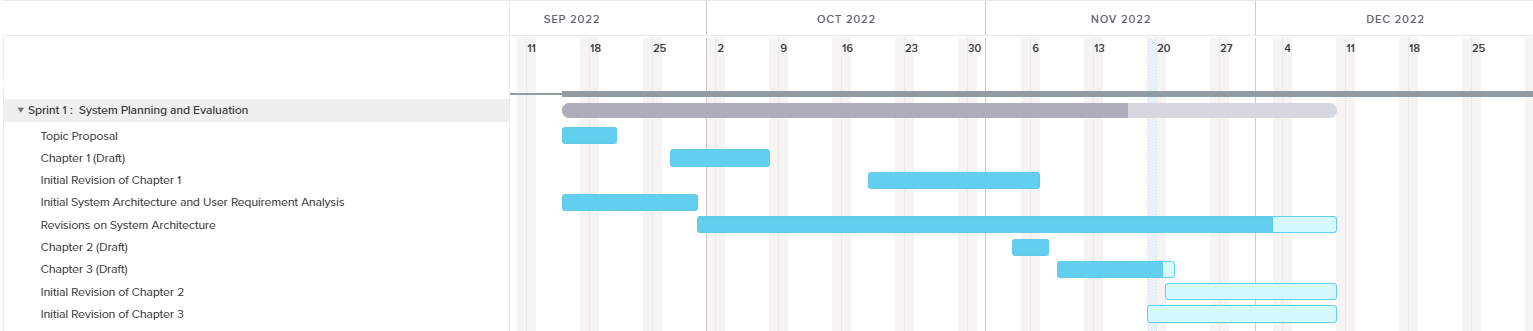
\includegraphics[width=1\textwidth]{./assets/Gantt_Chart_Sprint1.png}
    \caption{Gantt Chart for Sprint 1}
    \label{fig:gantt_chart_sprint1}
\end{figure}
\FloatBarrier}
% Gantt Chart for Sprint 2
\subsection{Gantt Chart for Sprint 2}
\label{subsec:gantt_chart_sprint2}
Figure \ref{fig:gantt_chart_sprint2} shows the schedule of activities 
for Sprint 2.
% Gantt Chart for Sprint 2
\begin{figure}[ht]
    \centering
    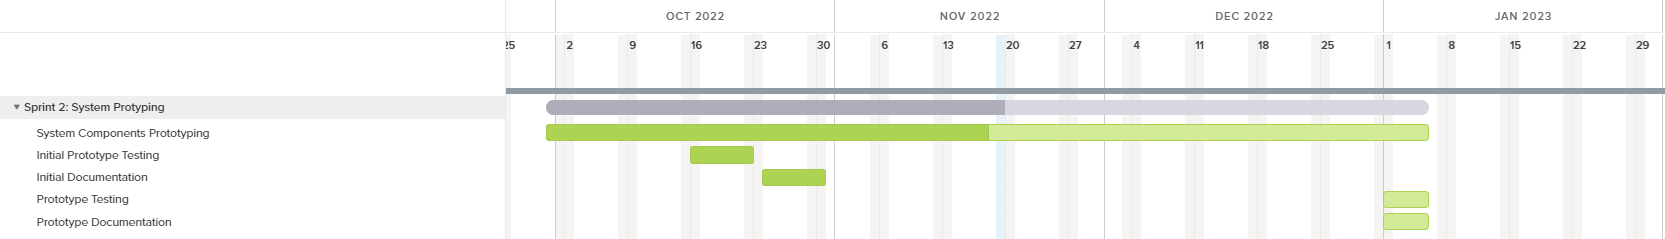
\includegraphics[width=0.80\textwidth]{./assets/Chapter_3/Gantt/Gantt_Chart_Sprint2.png}
    \caption{Gantt Chart for Sprint 2}
    \label{fig:gantt_chart_sprint2}
\end{figure}
\FloatBarrier
}
% Gantt Chart for Sprint 3
\subsection{Gantt Chart for Sprint 3}
\label{subsec:gantt_chart_sprint3}
Figure \ref{fig:gantt_chart_sprint3} shows the schedule of activities for Sprint 3. 
Wherein, it will start on January 15, 2023, and end on March 30, 2023.
% Gantt Chart for Sprint 3
\begin{figure}[ht]
    \centering
    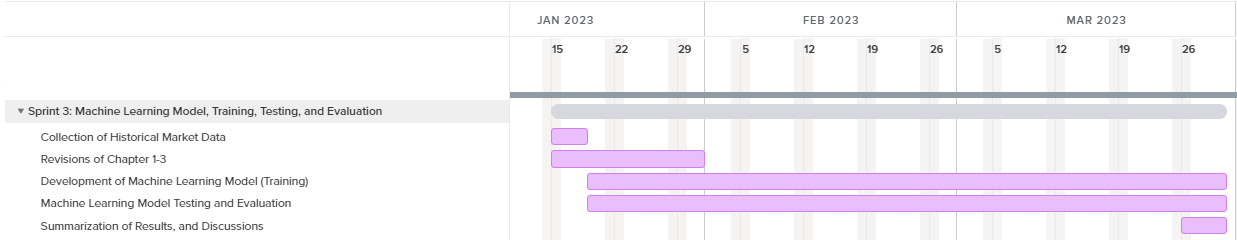
\includegraphics[width=1\textwidth]{./assets/Chapter_3/Gantt/Gantt_Chart_Sprint3.png}
    \caption{Gantt Chart for Sprint 3}
    \label{fig:gantt_chart_sprint3}
\end{figure}
\FloatBarrier}
% Gantt Chart for Sprint 4
\subsection{Gantt Chart for Sprint 4}
\label{subsec:gantt_chart_sprint4}
Figure \ref{fig:gantt_chart_sprint4} shows the schedule of activities for Sprint 4. 
Which will run from March 31, 2023, until May 12, 2023.
% Gantt Chart for Sprint 4
\begin{figure}[ht]
    \centering
    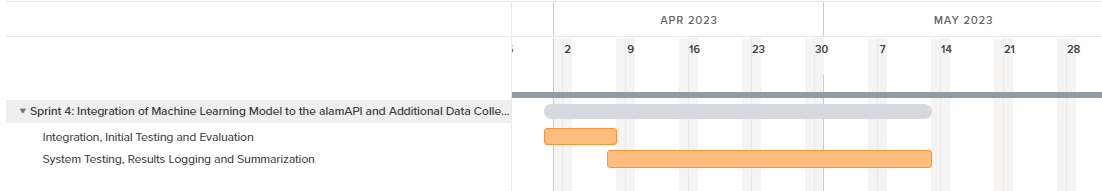
\includegraphics[width=1\textwidth]{./assets/Gantt_Chart_Sprint4.png}
    \caption{Gantt Chart for Sprint 4}
    \label{fig:gantt_chart_sprint4}
\end{figure}
\FloatBarrier}
% Gantt Chart for Sprint 5
\subsection{Gantt Chart for Sprint 5}
\label{subsec:gantt_chart_sprint5}
Figure \ref{fig:gantt_chart_sprint5} shows the schedule of activities for Sprint 5. 
% Gantt Chart for Sprint 5
\begin{figure}[ht]
    \centering
    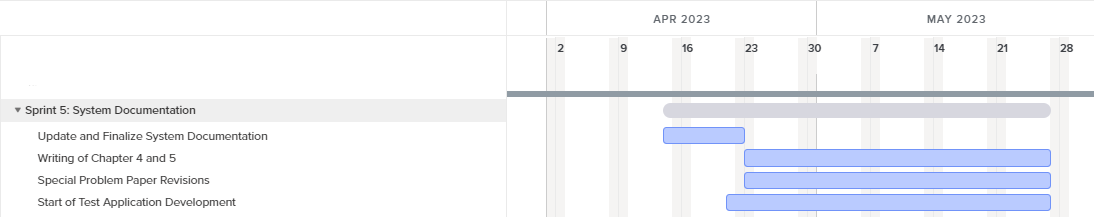
\includegraphics[width=1\textwidth]{./assets/Chapter_3/Gantt/Gantt_Chart_Sprint5.png}
    \caption{Gantt Chart for Sprint 5}
    \label{fig:gantt_chart_sprint5}
\end{figure}
\FloatBarrier}
% Gantt Chart for Sprint 6
\subsection{Gantt Chart for Sprint 6}
\label{subsec:gantt_chart_sprint6}
Figure \ref{fig:gantt_chart_sprint6} shows the schedule of activities for the final sprint 
for the development of alamSYS.
% Gantt Chart for Sprint 6
\begin{figure}[ht]
    \centering
    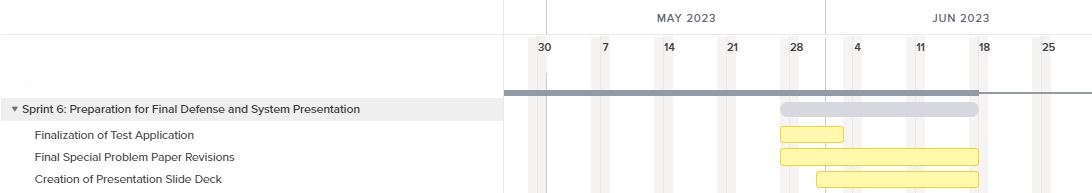
\includegraphics[width=1\textwidth]{./assets/Chapter_3/Gantt/Gantt_Chart_Sprint6.png}
    \caption{Gantt Chart for Sprint 6}
    \label{fig:gantt_chart_sprint6}
\end{figure}
\FloatBarrier}
% Full Gantt Chart
\subsection{Full Gantt Chart}
\label{subsec:gantt_chart_full}
To have an overview of the whole schedule of each Sprints, 
the full Gantt chart is shown in Figure \ref{fig:gantt_chart_full}.
% Full Gantt Chart
\begin{figure}[ht]
    \centering
    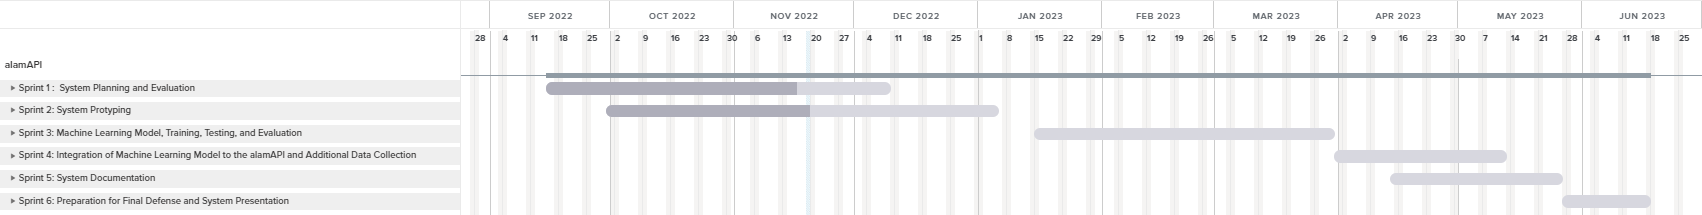
\includegraphics[width=1\textwidth]{./assets/Chapter_3/Gantt/Gantt_Chart_Full.png}
    \caption{Full Gantt Chart}
    \label{fig:gantt_chart_full}
\end{figure}
\FloatBarrier}